%%%%%%%%%%%%%%%%%%%%%%%%%%%%%%%%%%%%%%%%%%%%%%%%%%%%%%%%%%%%%%%
\section{Missing transverse energy}\label{sec:met}
%%%%%%%%%%%%%%%%%%%%%%%%%%%%%%%%%%%%%%%%%%%%%%%%%%%%%%%%%%%%%%%

CMS is a full coverage hermetic detector which identifies and reconstructs almost all stable or long-lived particles produced in pp collisions. 
The only exceptions are neutrinos and hypothetical neutral weakly interacting particles.
Although these particles do not leave a signal in the detector, their presence can be inferred from the momentum imbalance in the transverse plane,
a quantity known as missing transverse momentum and denoted by \ptvecmiss.

The standard method available in CMS for the reconstruction of \ptvecmiss uses the PF algorithm~\cite{1748-0221-6-09-P09001}.
%Several standard methods are available in CMS for the reconstruction of \ptvecmiss, which, as for the jet reconstruction, can be based on calorimeter information only, include also tracker information, or use the PF algorithm~\cite{1748-0221-6-09-P09001}. 
The PF \ptvecmiss is used in this analysis along with PF jets and it is calculated as the negative vector sum of the transverse momenta of all reconstructed PF candidates in a given event

\begin{equation}
\ptvecmiss = -\sum_{i}^{N}{\vec p}_{\mathrm{T},i}.
\end{equation}

Its magnitude is referred to as missing transverse energy and denoted by \ETmiss.
The \ETmiss is an important variable in many searches for physics beyond the standard model such as the ones described in this thesis where a real highly energetic neutrino is expected in the final state.
In addition, the precise measurement of \ETmiss plays a crucial role for measurements of standard model physics involving W bosons and top quarks.
The \ptvecmiss reconstruction is sensitive to pileup, detector malfunctions and to various reconstruction effects. A precise calibration of all reconstructed physics objects is therefore crucial for its performance.
The level of mismeasurement is significantly reduced after jet energy calibration, described in Section~\ref{subsec:jetsreco}.
A correction to the \ptvecmiss is derived by propagating the jet energy scale corrections as described in the following.

The raw missing transverse momentum can be written as:

\begin{equation}
{\vec p}_\mathrm{T}^\mathrm{\; miss,raw} = - \sum_{i}^{N_\mathrm{jets}} {\vec p}_{\mathrm{T},i}^{\;\mathrm{raw}} - \sum_{i}^{N_\mathrm{uncl}} {\vec p}_{\mathrm{T},i},
\end{equation}

where the first and second sum runs over the \pt of the PF candidates clustered as jets and unclustered, respectively, and the superscript ``raw'' indicates the uncorrected value.
The correction to the \ptvecmiss is then obtained by replacing the first sum with the vector sum of the transverse momenta of the jets to which jet energy scale corrections (JEC) are applied:

\begin{equation}
{\vec C}_\mathrm{T}^\mathrm{JEC} = \sum_{i}^{N_\mathrm{jets}} {\vec p}_{\mathrm{T},i}^{\;\mathrm{raw}} - \sum_{i}^{N_\mathrm{jets}} {\vec p}_{\mathrm{T},i}^{\;\mathrm{JEC}},
\end{equation}

where the sum is performed over all jets with corrected $\pt > 10\GeV$.

%Further corrections improve the performance of the \ptvecmiss reconstruction in events with large numbers of pileup interactions. This is achieved as explained in the following.
%
%The raw \ptvecmiss can be written as a sum of the two contributions due to particles produced in the primary vertex (PV) and in pileup interactions (PU)
%
%\begin{equation}\label{eqn:metraw}
%{\vec p}_\mathrm{T}^\mathrm{\; miss,raw} = - \sum_{i \in \mathrm{PV}} {\vec p}_{\mathrm{T},i} - \sum_{i \in \mathrm{PU}} {\vec p}_{\mathrm{T},i}.
%\end{equation}
%
%Particles produced in the pileup interactions can be further classified into neutral (PUneu) and charged (PUch) particles so that the equation above can be expressed as
%
%\begin{equation}
%{\vec p}_\mathrm{T}^\mathrm{\; miss,raw} = - \sum_{i \in \mathrm{PV}} {\vec p}_{\mathrm{T},i} - \sum_{i \in \mathrm{PUch}} {\vec p}_{\mathrm{T},i} - \sum_{i \in \mathrm{PUneu}} {\vec p}_{\mathrm{T},i}.
%\end{equation}
%
%The contribution to the genuine \ptvecmiss from such interactions is close to zero, as the probability to produce neutrinos is small in inelastic pp scattering interactions (e.g. neutrinos from Kaon decays).
%The vectorial \Vpt sum of charged particles is therefore expected to be well balanced by that of neutral particles.
%However, the nonlinearity and minimum energy thresholds in the calorimeters cause \ptvecmiss to point on average in the direction of the vectorial \Vpt sum of neutral particles.
%Nevertheless, it can be assumed that the directions of neutral pileup particles is measured with high precisions from the positions of the calorimeter cells in which we observe the energy deposits, while their energies are systematically off by the same factor. At the same time, the CMS tracker can also measure very well the charged pileup particles from their large curvature due to the low \pt characterizing this type of processes.
%With these assumptions, the total contribution from pileup can be estimated as
%
%\begin{equation}
%{\vec \Delta}_\mathrm{PU} = \sum_{i \in \mathrm{PUch}} {\vec p}_{\mathrm{T},i} + \sum_{i \in \mathrm{PUneu}} {\vec p}_{\mathrm{T},i} = \sum_{i \in PU} f({\vec v}) {\vec v},
%\end{equation}
%
%where ${\vec v}$ represents the sum of the transverse momenta of charged particles for each pileup interaction.
%The correction $f({\vec v})$ is parametrized as $f({\vec v}) = c_1 (1.0 +erf(-c_2|{\vec v}^{c_3}|))$, where the coefficients $c_1$, $c_2$, and $c_3$ are extracted from simulated minimum bias events.
%The corrected \ptvecmiss is then obtained removing the additional contribution ${\vec \Delta}_\mathrm{PU}$ from Eq.~\ref{eqn:metraw}
%
%\begin{equation}
%{\vec p}_\mathrm{T}^\mathrm{\; miss,PUcorr} = {\vec E}_\mathrm{T}^\mathrm{\; miss,raw} + {\vec \Delta}_\mathrm{PU}.
%\end{equation}
%
Another type of correction is derived and applied to correct for a modulation in $\phi$ in the \ptvecmiss present not only in data but also in simulation. The distribution of genuine \ptvecmiss is instead independent of $\phi$ because of the rotational symmetry of the collisions around the beam axis. The possible causes of the modulation include imperfect detector alignment, inefficiencies, a residual \pt dependence of the calibration, and a shift between the center of the detector and the beam line. The correction for this effect can be expressed as a shift in the \ptvecmiss components along the $x$ and $y$ detector coordinates, which increases approximately linearly with the number of reconstructed vertices. This correlation is used for a correction procedure as follows

\begin{equation}
{\vec E}_{\mathrm{T},x}^\mathrm{\; miss,\phi corr} = {\vec E}_{\mathrm{T},x}^\mathrm{\; miss,raw} - (c_{x_0} + c_{x_s}N_\mathrm{vtx}),\\
{\vec E}_{\mathrm{T},y}^\mathrm{\; miss,\phi corr} = {\vec E}_{\mathrm{T},y}^\mathrm{\; miss,raw} - (c_{y_0} + c_{y_s}N_\mathrm{vtx}),
\end{equation}

where the coefficients are determined separately for data and simulated events.
%Other more sophisticated missing energy determinations aimed at improving the resolution have been developed in CMS\cite{Khachatryan:2014gga,CMS-PAS-JME-16-004} but will not be discussed in this section since they are not used in this work.\\

The distributions of the PF \ETmiss, obtained after applying all the corrections described above, in $\PZ\to\MM$, $\PZ\to\EE$, and prompt photon events are presented in Fig.~\ref{fig:met_distr} as measured in 8\TeV data and for simulation. Good agreement between data and simulation is observed in all distributions.

These events contain no genuine \ptvecmiss, and thus a balance exists between the well-measured vector boson transverse momentum, denoted as ${\vec q}_\mathrm{T}$, and the hadronic recoil, denoted as ${\vec u}_\mathrm{T}$,  which dominates the \ptvecmiss measurement. The $q_\mathrm{T}$ can therefore be used as a reference to measure the scale and resolution of \ptvecmiss.
The hadronic recoil can be projected to the axis defined by $q_\mathrm{T}$, yeilding two signed components, parallel ($u_\parallel$) and perpendicular ($u_\perp$) to this axis. The parallel component is typically negative as the observed hadronic system is usually in the hemisphere opposite the boson. The scalar quantity $-\left\langle u_\parallel\right\rangle/{\vec q}_\mathrm{T}$ is referred to as the \ptvecmiss response. The response curves, extracted from the data as a function of the vector boson boost ${\vec q}_\mathrm{T}$, are shown in Fig.~\ref{fig:met_resol_a}, where deviations from unity indicate a bias on the hadronic recoil energy scale which is  fully recovered for ${\vec q}_\mathrm{T} > 40\GeV$.
%The bias is fully recovered for ${\vec q}_\mathrm{T} > 40\GeV$, while below this value the uncorrected unclustered energy contribution starts to be significant compared to the corrected energy of the recoiling jets, leading to an underestimation of the response.
%A reasonable agreement is found between data and simulation.
%The curves fit to $\gamma$ + jets data are 2?3\% lower than those fit to Z data at ${\vec q}_\mathrm{T} < 100\GeV$. This effect primarily stems from the large contribution of QCD multijet events to the ${\vec q}_\mathrm{T} < 100\GeV$ region of the selected photon sample. In these QCD multijet events, the hadronic recoil of the photon candidate tends to have a higher contamination of gluon jets. As the calorimeter response to gluon jets is characteristically lower than for quark jets due to difference of jet composition and collimation, the overall average response is reduced for the photon sample in this region.
The resolution curves, $\sigma(u_\parallel)$ and $\sigma(u_\perp)$ as a function of $q_\mathrm{T}$, are shown in Fig.~\ref{fig:met_resol_b} and~\ref{fig:met_resol_c}, respectively, for each control sample. The resolution increases with increasing $q_\mathrm{T}$, while the data and simulation curves are in good agreement for each control sample.\\

\begin{figure}[!htb]
\begin{center}
\subfigure[]{\label{fig:met_distr_a}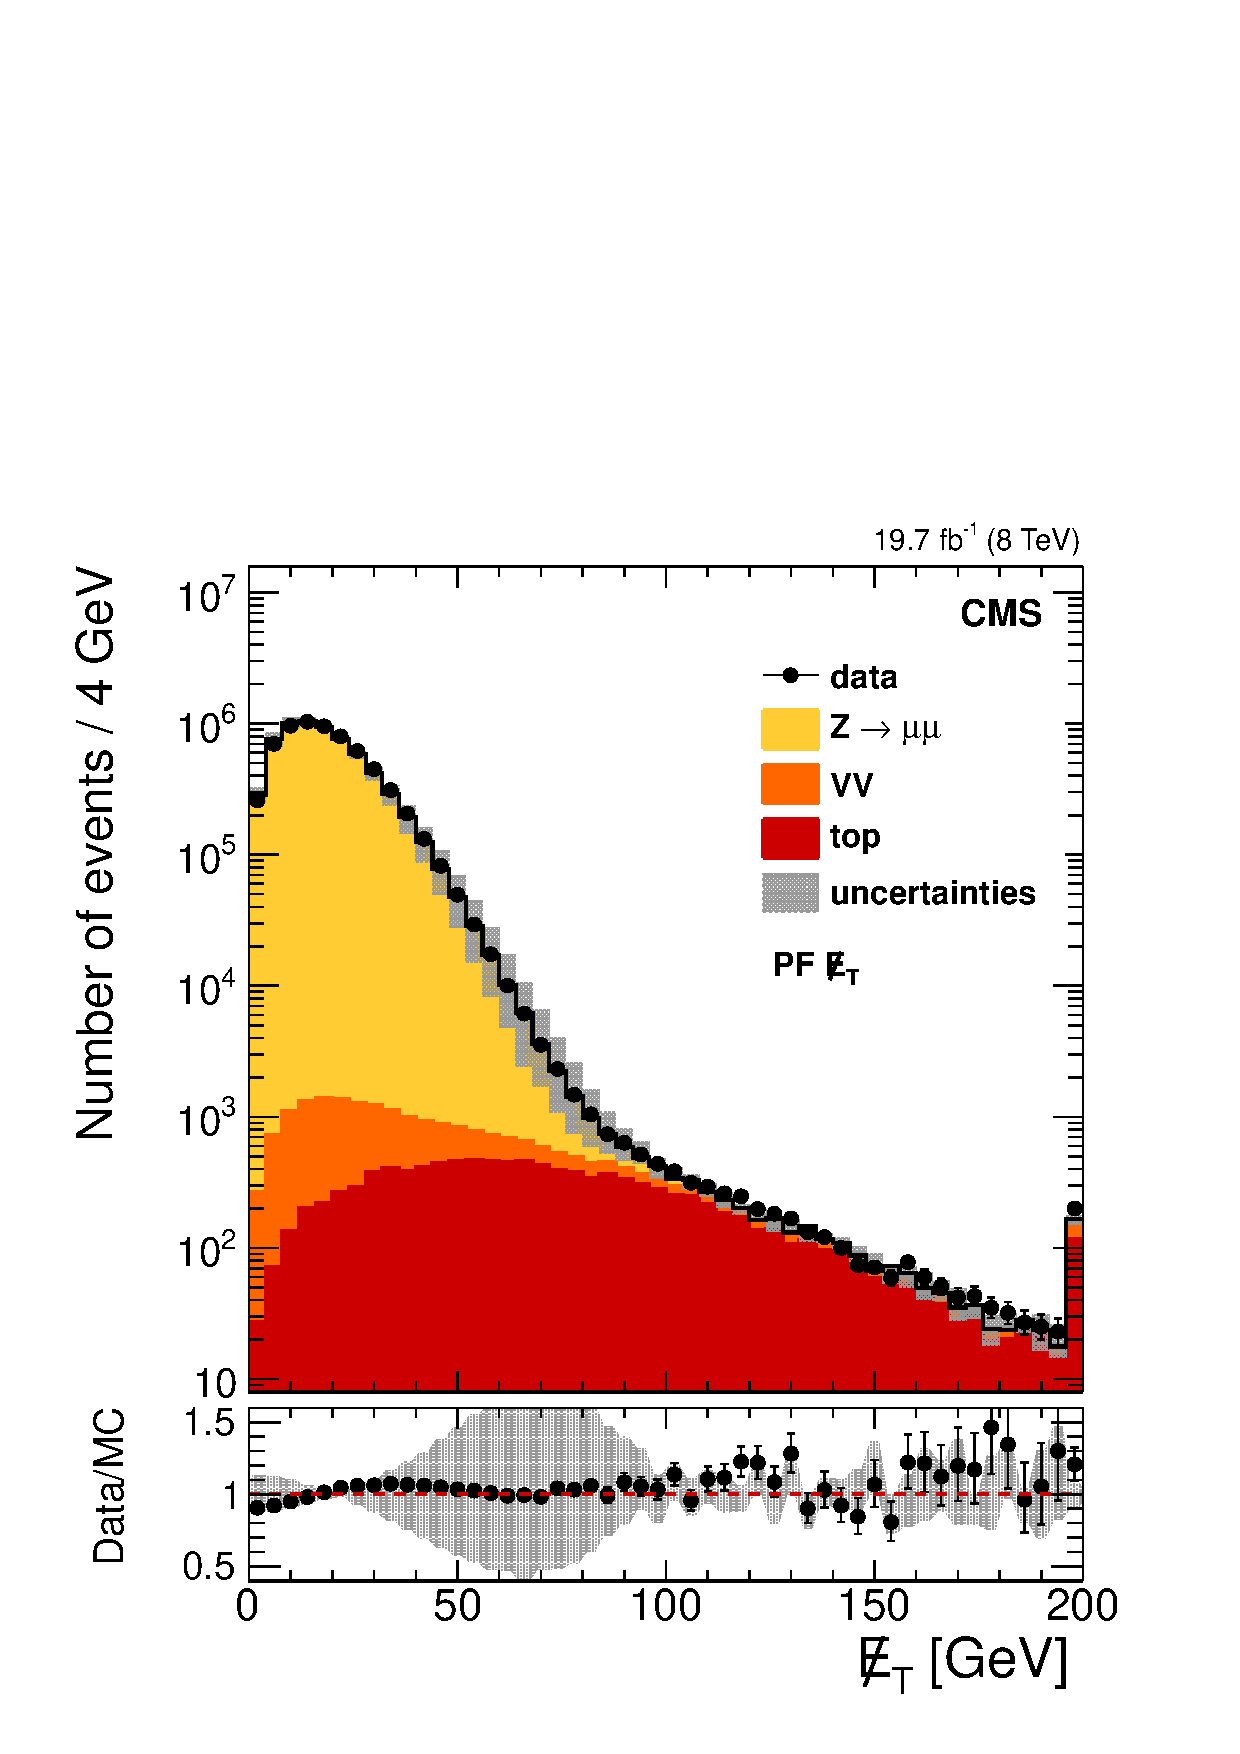
\includegraphics[width=0.3\textwidth]{\chsix/met-run1-type1phi-zmm.pdf}}
\subfigure[]{\label{fig:met_distr_b}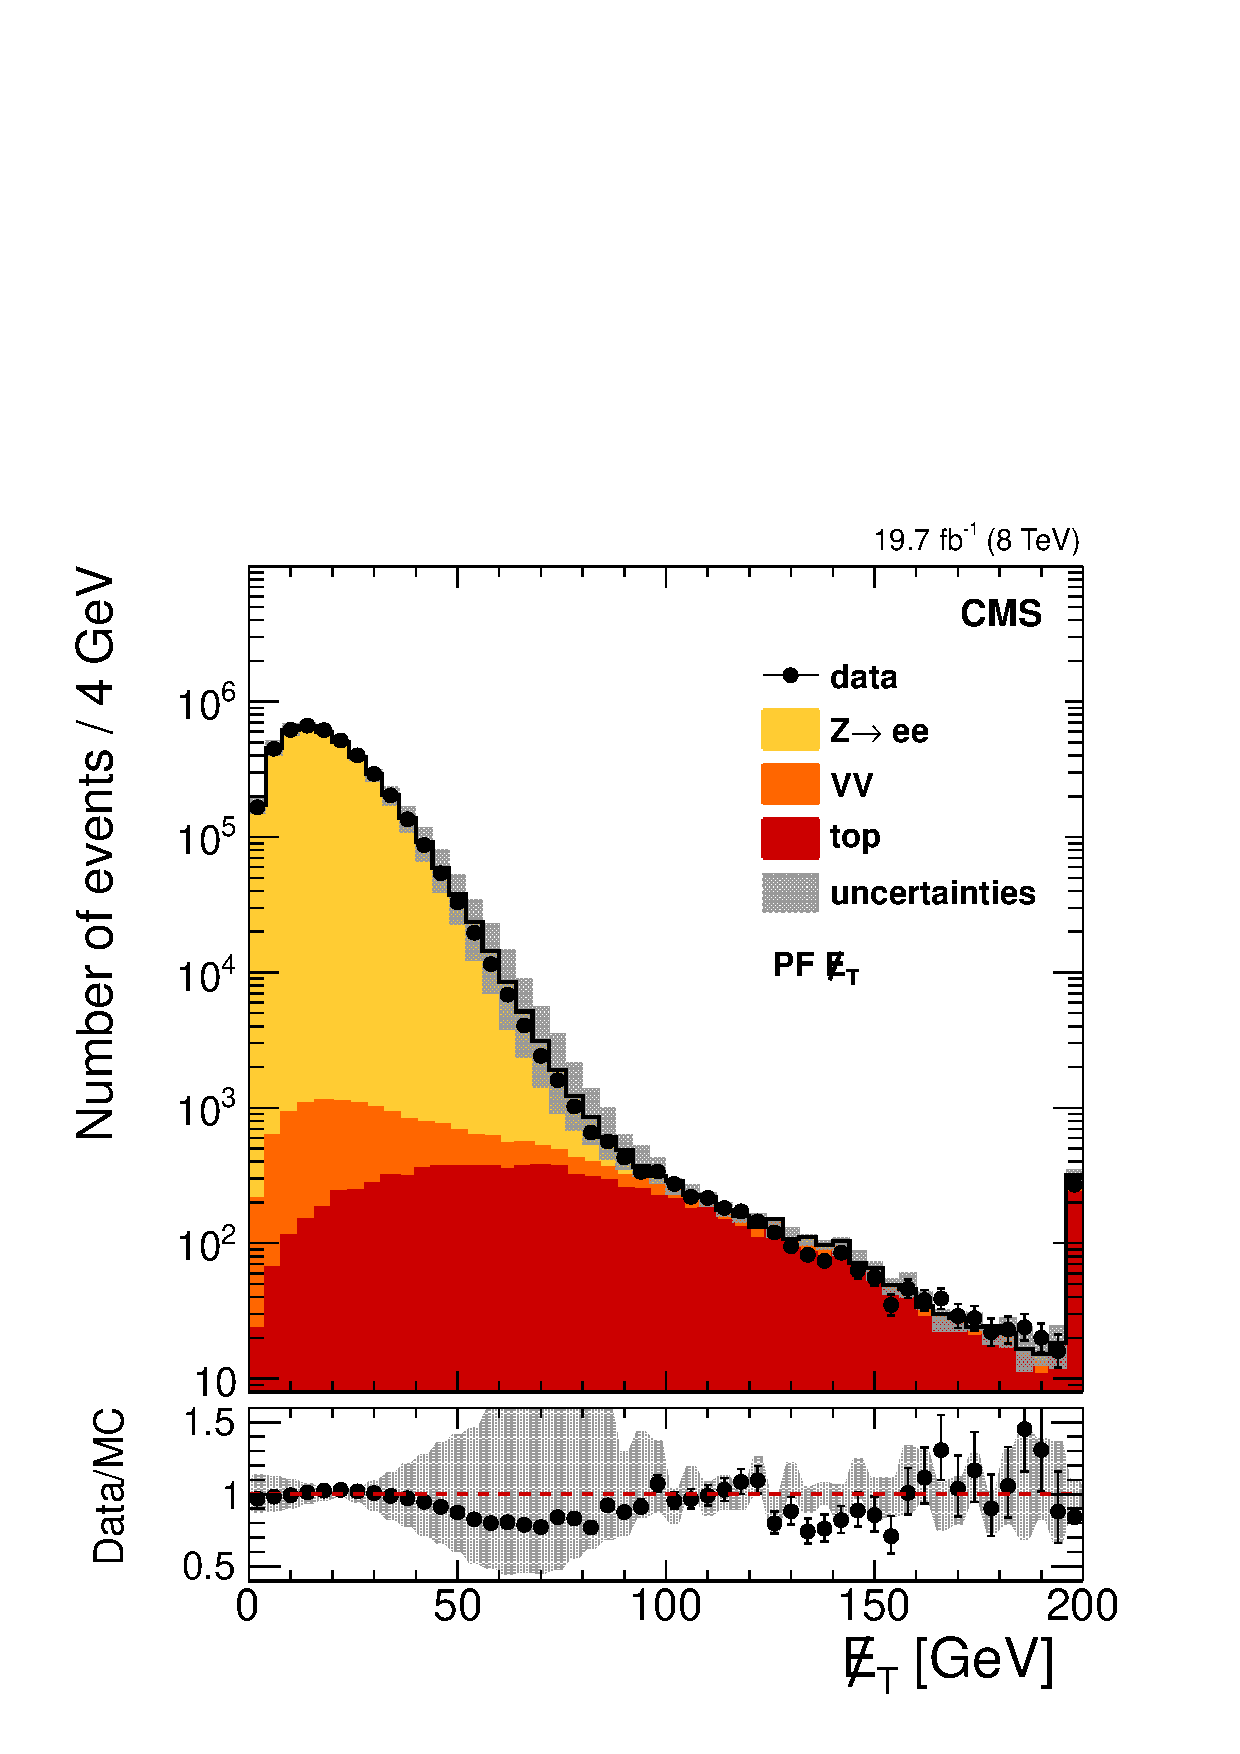
\includegraphics[width=0.3\textwidth]{\chsix/met-run1-type1phi-zee.pdf}}
\subfigure[]{\label{fig:met_distr_c}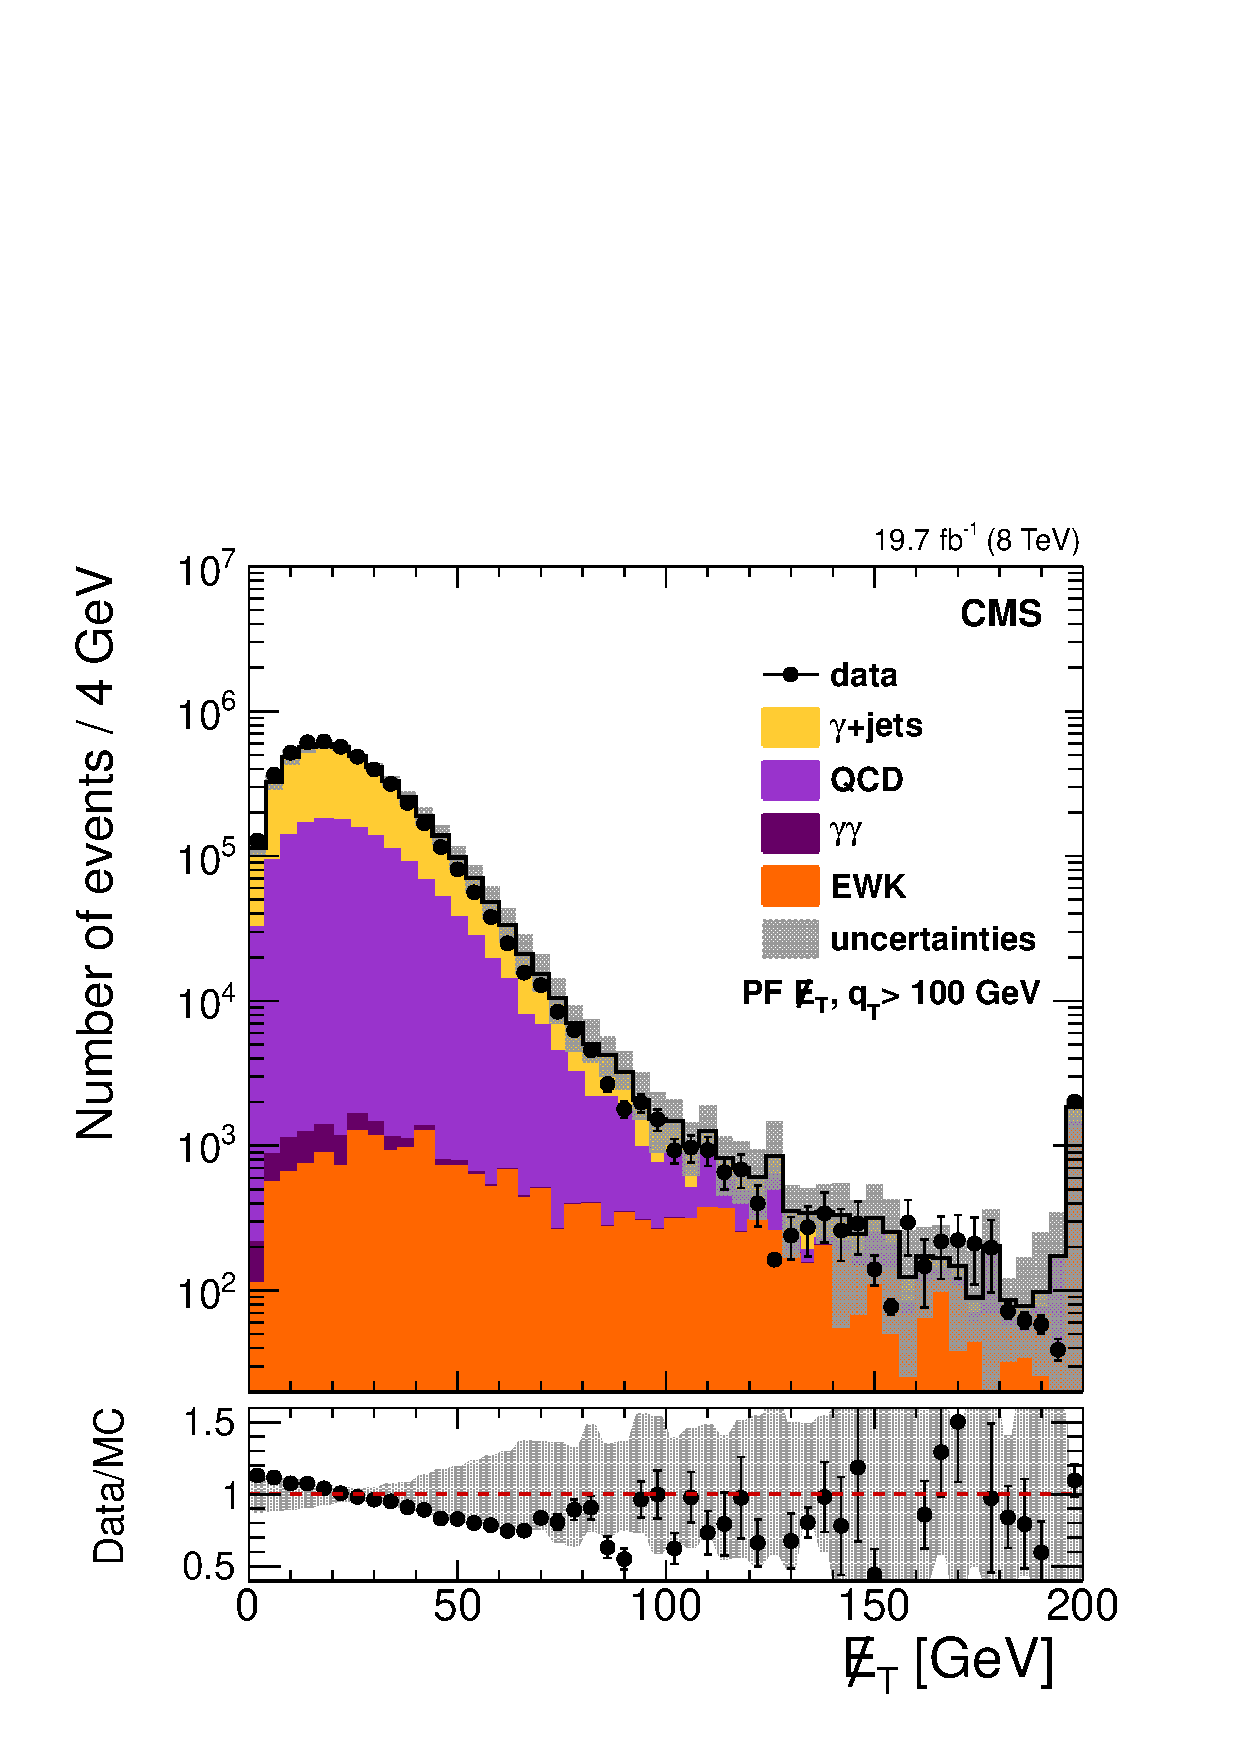
\includegraphics[width=0.3\textwidth]{\chsix/met-run1-type1phi-zgg.pdf}}
\end{center} 
\caption{The PF \ETmiss distribution in $\PZ\to\MM$ (a), $\PZ\to\EE$ (b), and prompt photon (c) events for 8\TeV data and for simulation. The points in the lower panel of each plot show the ratio between data and simulation describing their agreement~\cite{Khachatryan:2014gga}.}
\label{fig:met_distr}
\end{figure}

\begin{figure}[!htb]
\begin{center}
\subfigure[]{\label{fig:met_resol_a}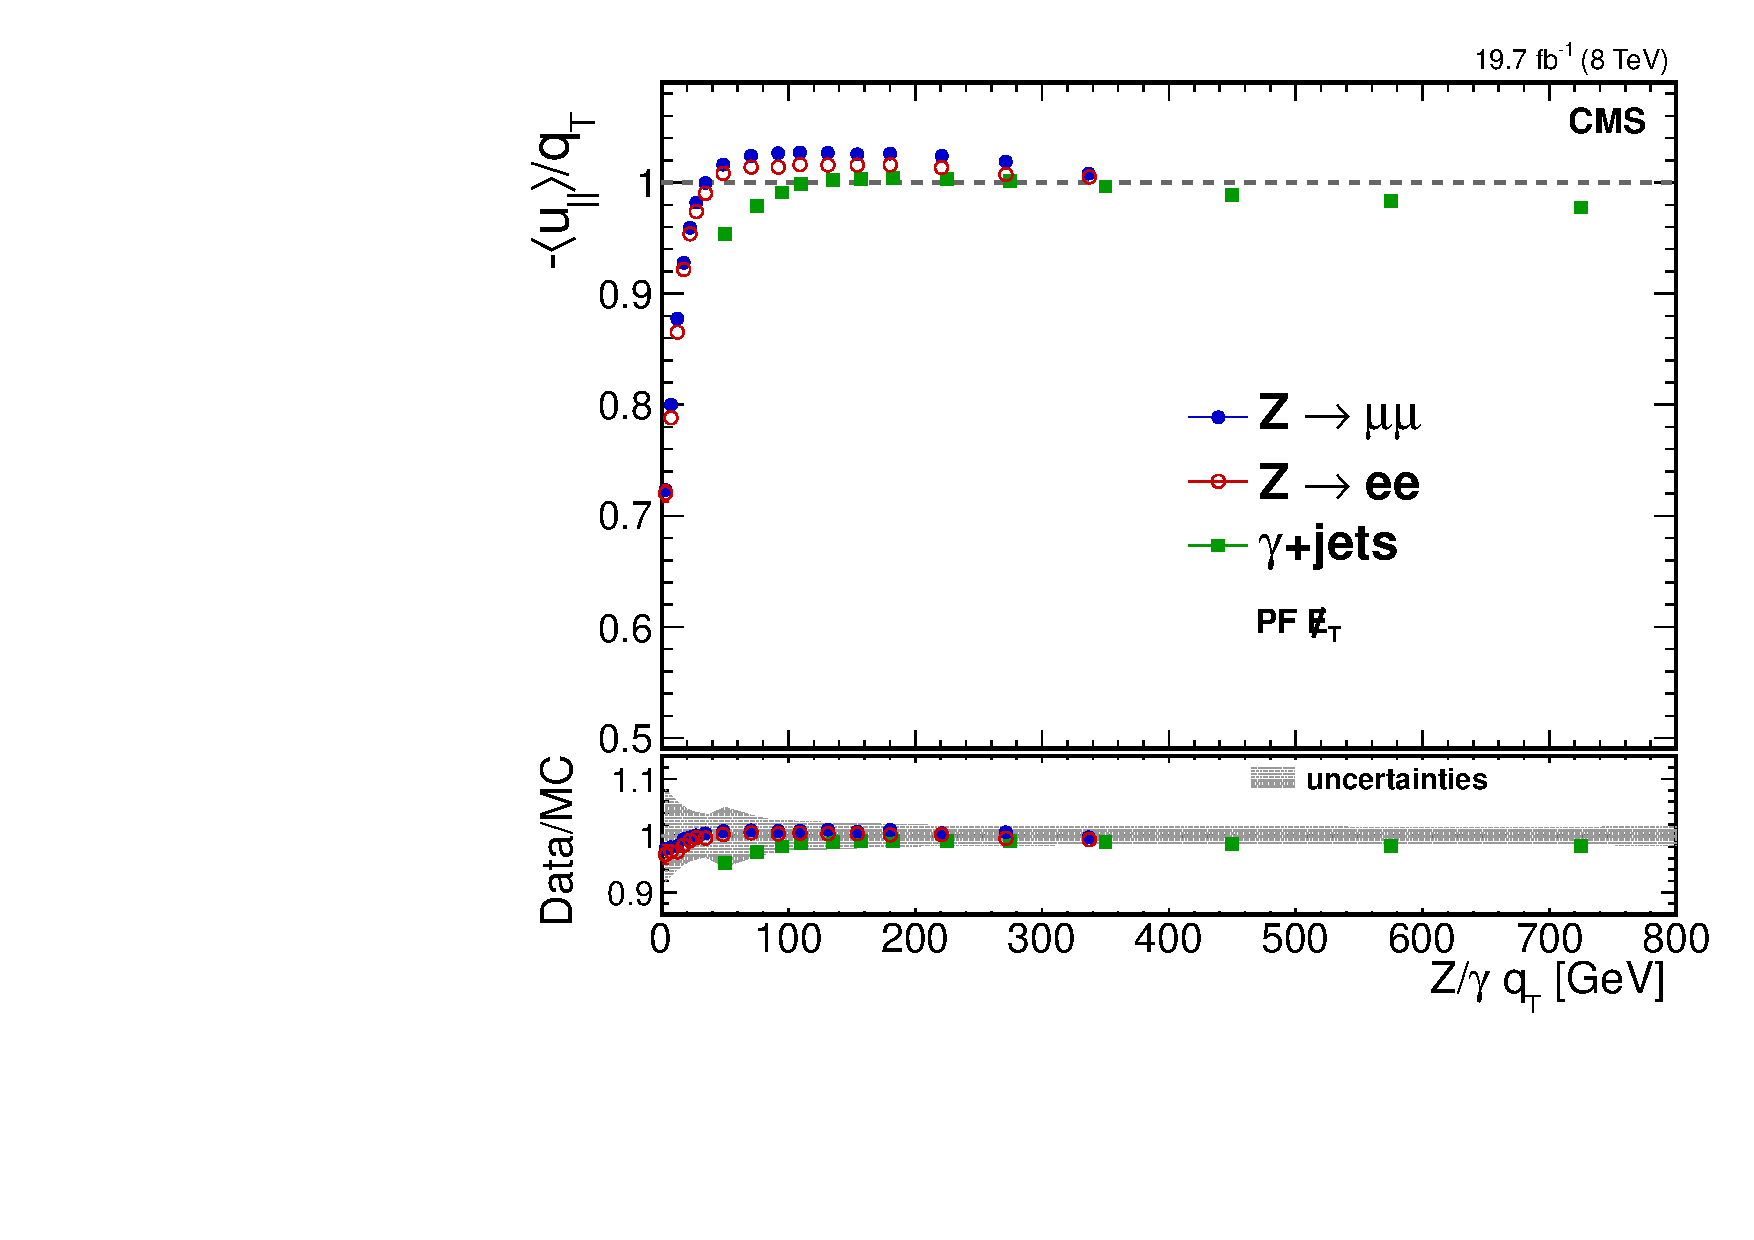
\includegraphics[width=0.3\textwidth]{\chsix/met-run1-type1phi-resp.pdf}}
\subfigure[]{\label{fig:met_resol_b}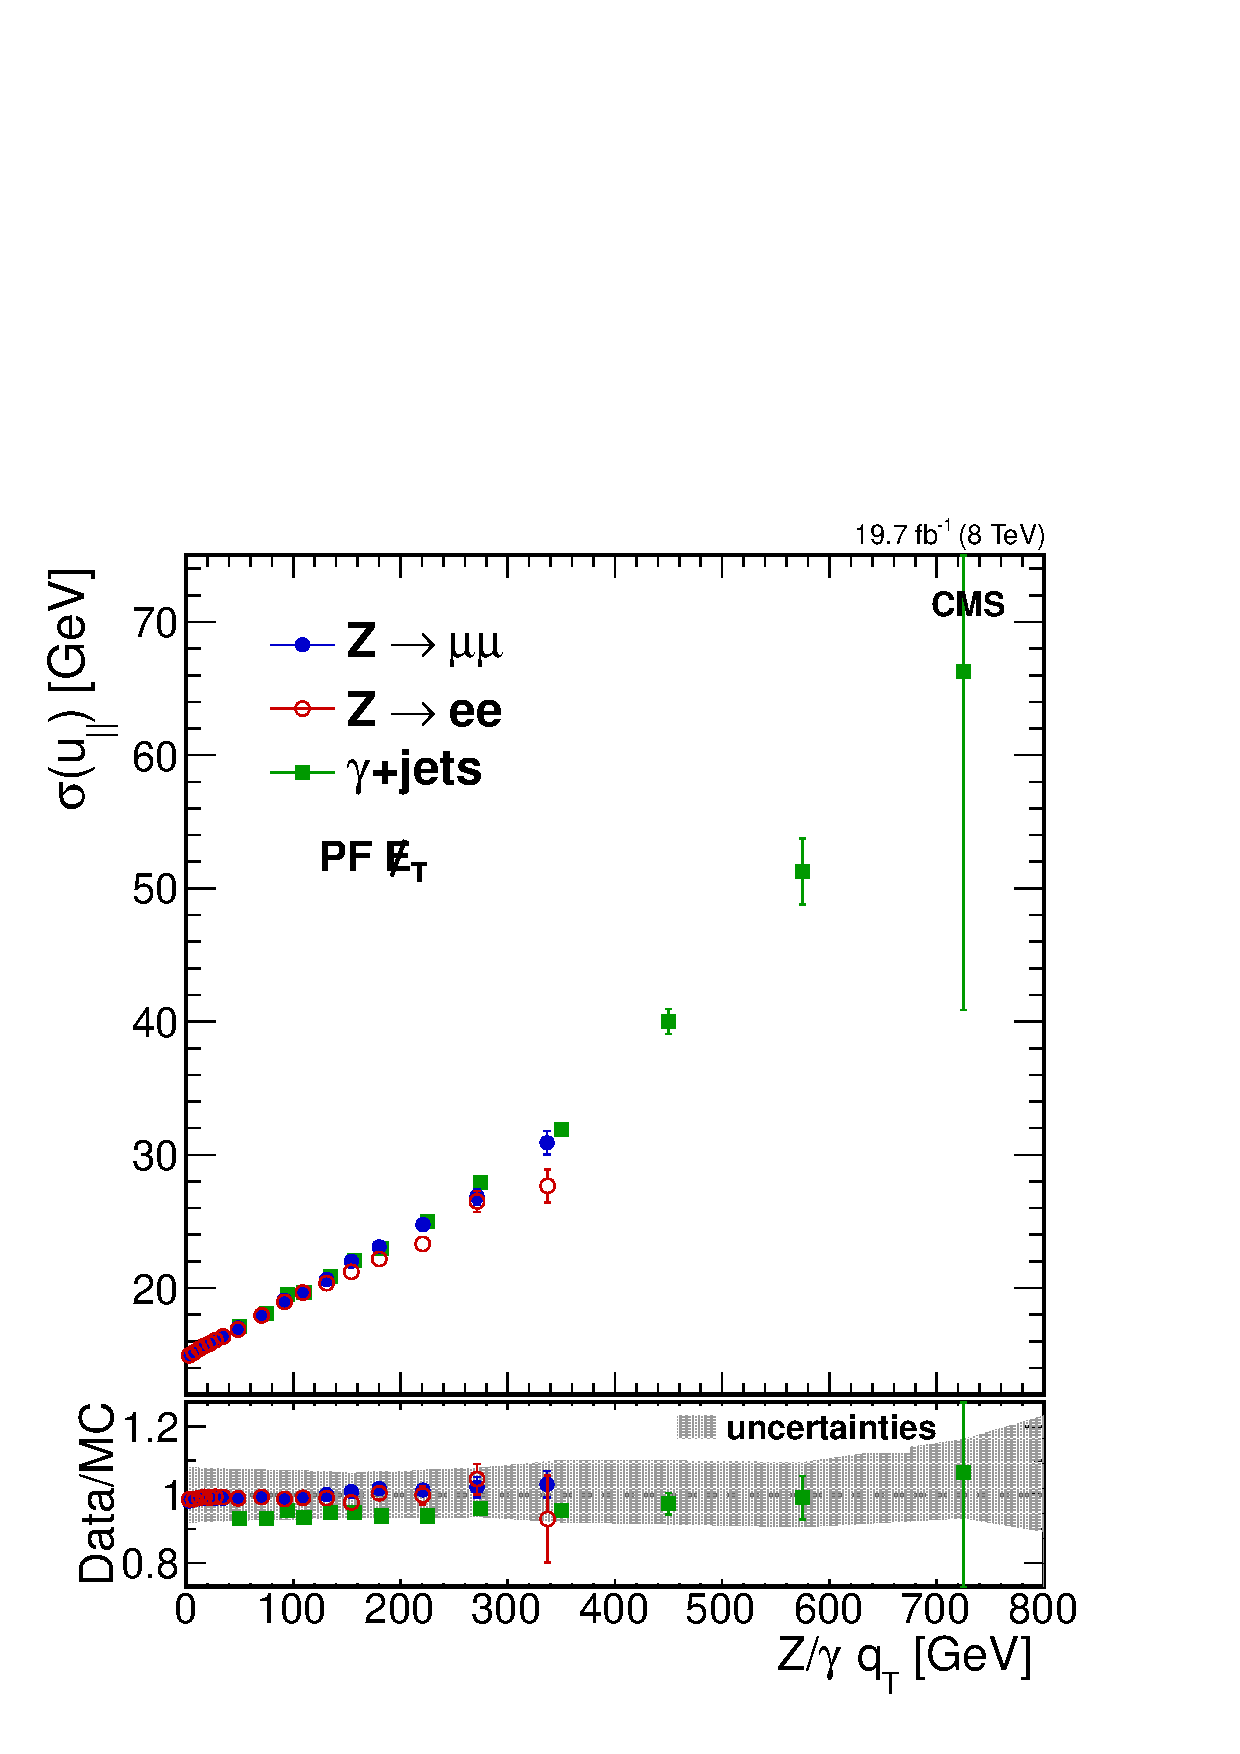
\includegraphics[width=0.3\textwidth]{\chsix/met-run1-type1phi-resopara.pdf}}
\subfigure[]{\label{fig:met_resol_c}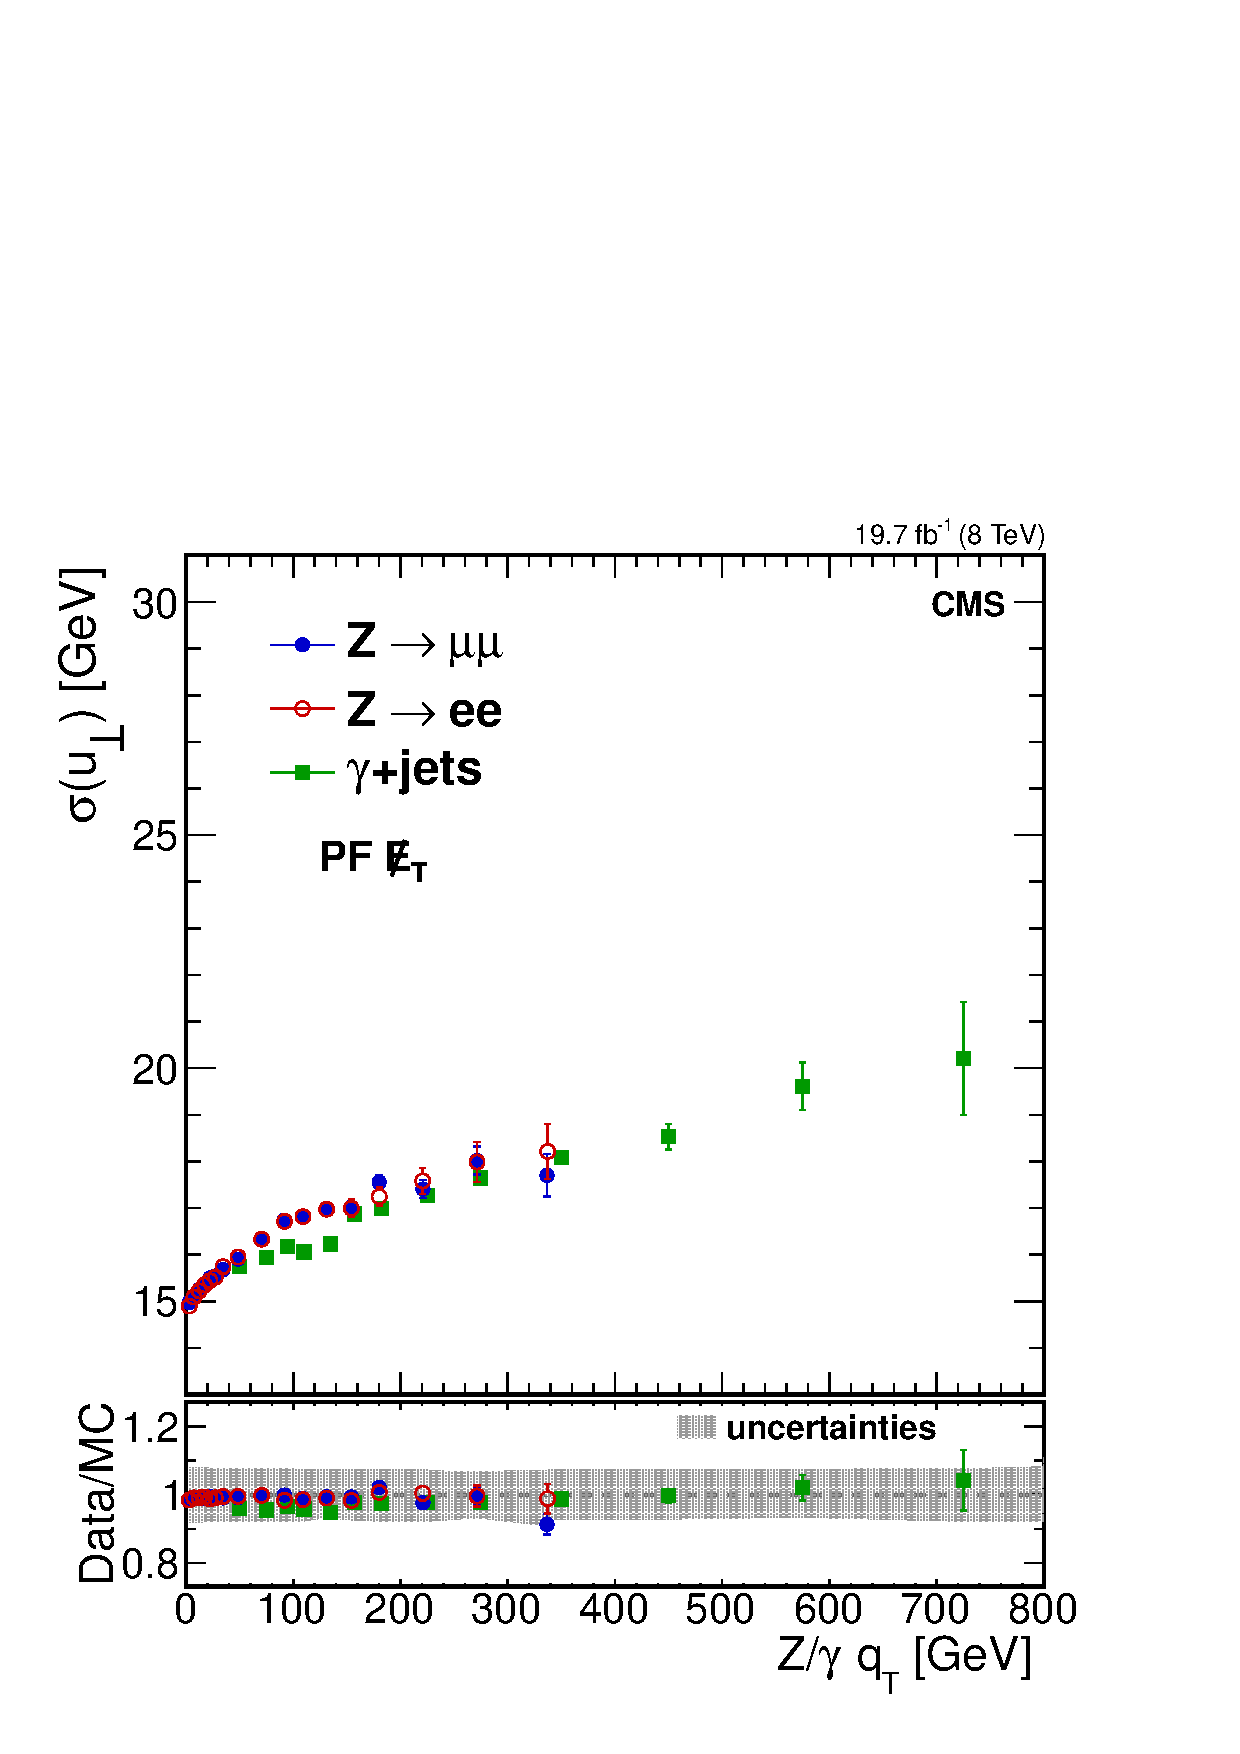
\includegraphics[width=0.3\textwidth]{\chsix/met-run1-type1phi-resoperp.pdf}}
\end{center} 
\caption{(a) Response curves for PF \ptvecmiss in events with a Z-boson or prompt photon.
Also shown are the resolution curves of the parallel (b) and perpendicular (b) recoil components as a function of the Z/$\gamma$ $q_\mathrm{T}$. 
In each plot the upper frame shows the response in 8\TeV data, while the lower one shows the ratio between data and simulation.~\cite{Khachatryan:2014gga}.}
\label{fig:met_resol}
\end{figure}
